
\section{黄金比例}
\label{sec:golden-ratio}

\begin{definition}
  将线段分为长短两截,若短的一截比长的一截等于长的一截比原线段的长度,则此分割为\term{黄金分割}。
\end{definition}

记原线段长度为L,在黄金分割下,长一截长度为$l$,短的一截长度为$s$,则
\begin{align*}
  &\frac sl=\frac lL,\quad l+s=L\\
  \implies& \frac sl=\frac l{l+s}
\end{align*}
从而有
\begin{align*}
  \frac ls=\frac{\sqrt5+1}2\approx 1.618, \quad \frac sl=\frac{\sqrt5-1}2\approx 0.618
\end{align*}
以上两个常数都称为\term{黄金比例},通常用$\phi$和$\Phi$表示,即
\begin{align*}
  \phi\equiv\frac{\sqrt5+1}2,\quad \Phi\equiv\frac{\sqrt5-1}2
\end{align*}

\begin{question}
  证明下列恒等式:
  \begin{align*}
    \phi\cdot\Phi=1,\quad \phi=\Phi+1,\quad \phi^2=\phi+1,\quad \frac1\phi=\phi-1
  \end{align*}
\end{question}

\begin{example}[连分数表示]\label{ex:phi-of-continued-fraction}
  \begin{align}
    \phi = 1 + \dfrac1{1 + \dfrac1{1+\dfrac1{1+\dfrac1{1+\cdots}}}}
  \end{align}
\end{example}
\begin{proof}
  利用$\phi=1+\dfrac1\phi$,设连分数为$x$,则
  \begin{align*}
    \frac1{x-1}=x\implies x^2-x-1=0\implies x=\frac{1\pm\sqrt5}2
  \end{align*}
  由$x>0$可知$x=\dfrac{1+\sqrt5}2=\phi$。
\end{proof}

\begin{definition}
  以下数值称为\term{贵金属分割}:
  \begin{align}
    \frac{n+\sqrt{n^2+4}}2,\quad\quad n=1,2,3,\cdots
  \end{align}
  当$n=1$时为黄金分割$\dfrac{\sqrt5+1}2$;当$n=2$时为\term{白银分割}$\sqrt2+1$;当$n=3$时为\term{青铜分割}$\dfrac{\sqrt{13}+3}2$。
\end{definition}
\begin{question}
  证明:贵金属分割都可以用以下的连分数形式表示
  \begin{align*}
    \frac{n+\sqrt{n^2+4}}2=
    n+\dfrac1{n+\dfrac1{n+\dfrac1{n+\dfrac1{n+\dfrac1{n+\cdots}}}}}
  \end{align*}
\end{question}

\begin{example}[平方根表示]
  \begin{align}
    \phi=\sqrt{1+\sqrt{1+\sqrt{1+\sqrt{1+\sqrt{1+\cdots}}}}}
  \end{align}
\end{example}
\begin{proof}
  记等号右边为$x$,则$x^2 = 1 + x$,余下与题~\ref{ex:phi-of-continued-fraction}相同,略。
\end{proof}

\begin{example}[三角函数表示]
  $\phi=1 + 2\sin18^\circ.$
\end{example}
\begin{proof}
  由$\phi=1+\Phi$,等价于证明$\sin18^\circ=\dfrac\Phi2$。令$x\equiv18^\circ$,则$2x+3x=5x=90^\circ$,应用以下公式
  \begin{align*}
    \sin 2x &= \cos \left(\frac\pi2 - 2x\right) = \cos 3x\\
    \sin 2x &=2\sin x\cos x\\
    \cos 3x &= 4\cos^3x-3\cos x
  \end{align*}
  可得
  \begin{align*}
    &2\sin x\cos x = 4\cos^3x-3\cos x\\
    \implies& \cos x(2\sin x - 4\cos^2 x + 3) = 0  & (cos x\ne 0)\\
    %\overset{\cos x\ne 0}{\implies} & 2\sin x + 4\sin^2 x - 1 = 0
    \implies & 2\sin x + 4\sin^2 x - 1 = 0 
  \end{align*}
  从而有
  \begin{align*}
    \sin x = \dfrac{-2\pm\sqrt{20}}{8}=\dfrac{-1\pm\sqrt5}4
  \end{align*}
又$x=18^\circ$,显然$\sin x>0$,从而有
\begin{align*}
  \sin18^\circ&=\sin x =\dfrac{\sqrt5-1}4=\dfrac\Phi2\qedhere
\end{align*}
\end{proof}

\begin{example}[黄金长方形]
  长宽比满足黄金比例的长方形称为\term{黄金长方形},如下图。\par
  \begin{center}
    \begin{tikzpicture}[scale=2.5];
      \draw(0,0)rectangle($({.5*(sqrt(5)+1)},1)$);
    \end{tikzpicture}
  \end{center}
\end{example}

\begin{example}[尺规作图]
  找出线段$AB$的黄金分割点。
\end{example}
关键点在于作出$\sqrt5$的长度,作出一个边长分别为$1,2,\sqrt5$的直角三角形。这里取$AB$的长度为$2$,则
\begin{enumerate}
\item 找出$AB$的中点$O$,则$AO=BO=1$;
\item 以$AO$为长度在过点$B$的$AB$垂直线上找点$C$,使$BC=AO=1$,则$AC=\sqrt5$;
\item 在$AC$上找点$D$,使$DC=BC=1$,此时$AD=\sqrt5-1$;
\item 在$AB$上找点$S$,使$AS=AD=\sqrt5-1$,从而$\dfrac{AS}{AB}=\dfrac{\sqrt5-1}{2}$,即点$S$是$AB$的黄金分割点。
\end{enumerate}
% \begin{figure}[htbp]
\begin{center}
  % \centering%\fbox{
  \vspace*{-5cm}
  \begin{tikzpicture}[scale=3]
    \coordinate[label=below left:$A$] (A) at (0,0);
    \coordinate[label=below right:$B$] (B) at (2,0);
    \coordinate[label=above:$C$] (C) at (2,1);
    \coordinate (O) at (1,0);
    \tkzInterLC(A,C)(C,B)\tkzGetPoints{D}{};
    \tkzInterLC(A,B)(A,D)\tkzGetPoints{}{S}\tkzLabelPoints[below](O,S)
    \calcLength(A,D){AD}
    %\draw(S) arc(0:40:\AD pt);
    \tkzMarkRightAngle[color=blue](A,B,C)
    \drawArc(A,S,D)
    \draw(A)--(O) node[midway,sloped]{||} -- (B)--(C) node[midway,sloped]{||}--(D)node[midway,sloped]{||} --cycle;
    % \draw(B) arc(270:200:1);
    \drawArc(C,B,D);
    \tkzDrawPoints(A,B,C,O,D,S);

    \clip(-1,0)rectangle(3,1);
  \end{tikzpicture}
%}
\end{center}
%   \caption{黄金分割的尺规作图}
%   \label{fig:golden-ratio-of-ruler-and-compass-construction}
% \end{figure}

\begin{definition}
  腰与底边的长度比是$\phi$的等腰三角形称为\term{黄金三角形}。
\end{definition}
\note 有时把腰与底边的长度比是$\Phi$的等腰三角形也称为黄金三角形。但此处只考虑比值是$\phi$的情况,即腰比底长的等腰三角形。


\begin{definition}
  等腰三角形的一条底角平分线将三角形分为两个三角形,若含底边的小三角形与原三角形相似,则称原三角形为\term{黄金三角形}。
\begin{center}
    \begin{tikzpicture}[scale=1];
      \begin{scope}[shift={(0,0)}]
        \coordinate(A) at (0,0);
        \coordinate(C) at (72:4);
        \coordinate(B) at ($(C)!1!36:(A)$); %rotate A to 36 degree around C
        \tkzDefLine[bisector](C,A,B)\tkzGetPoint{D'}
        \tkzInterLL(A,D')(B,C)\tkzGetPoint{D}
        \draw(A)--(B)node[midway,sloped]{|}--(C)node[midway,sloped]{||}--cycle node[midway,sloped]{||}--(D)node[midway,sloped]{|};
        \draw pic["$\theta$",<->,draw=orange,angle eccentricity=1.6,angle radius=.6cm]{angle=D--A--C};
        \draw pic["$\theta$",<->,draw=orange,angle eccentricity=1.6,angle radius=.6cm]{angle=B--A--D};
        \draw pic["$\theta$",<->,draw=orange,angle eccentricity=1.6,angle radius=.6cm]{angle=A--C--B};
        \draw pic["$2\theta$",<->,draw=orange,angle eccentricity=1.8,angle radius=.3cm]{angle=C--B--A};
        \draw pic["$2\theta$",<->,draw=orange,angle eccentricity=1.8,angle radius=.3cm]{angle=A--D--B};
        \tkzLabelPoints[below left](A)
        \tkzLabelPoints[below right](B)
        \tkzLabelPoints[above](C)
        \tkzLabelPoints[above right](D)
      \end{scope}
      \begin{scope}[shift={(5,0)}]
        \coordinate(A) at (0,0);
        \coordinate(C) at (72:4);
        \coordinate(B) at ($(C)!1!36:(A)$); %rotate A to 36 degree around C
        \tkzDefLine[bisector](C,A,B)\tkzGetPoint{D'}
        \tkzInterLL(A,D')(B,C)\tkzGetPoint{D}
        \draw(A)--(B)node[midway,sloped,below]{$\phi$}
                --(D)node[pos=.55,right]{$1$}
                --(C)node[midway,right]{$\phi$}
                --(A)node[midway,sloped,above]{$\phi^2=\phi+1$}
                --(D)node[pos=.55,above]{$\phi$};
        \tkzLabelPoints[below left](A)
        \tkzLabelPoints[below right](B)
        \tkzLabelPoints[above](C)
        \tkzLabelPoints[above right](D)
      \end{scope}
    \end{tikzpicture}
  \end{center}
\end{definition}

\begin{theorem}
  一个等腰三角形是黄金三角形的充要条件是其顶角是$\dfrac\pi5(36^\circ)$。
\end{theorem}
\begin{proof}
  必要性:由图,$5\theta=\pi$,从而$\theta=\dfrac\pi5$。

  充分性:若等腰三角形顶角$\angle C=\dfrac\pi5$,则容易计算到到$\angle BAD=\dfrac\pi5$,从而$\triangle ABC\sim\triangle BAD$,即$\triangle ABC$是黄金三角形。
\end{proof}

\begin{question}
  证明黄金三角形各边长度的比例关系如上图所示。
\end{question}

\begin{question}
  证明正五角星(Regular Pentagram)的顶点可组成黄金三角形。
  \begin{center}
    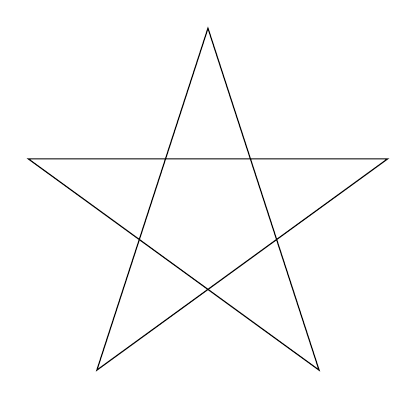
\begin{tikzpicture}[scale=.6]
      \coordinate(A) at ( 18:4);
      \coordinate(B) at ( 90:4);
      \coordinate(C) at (162:4);
      \coordinate(D) at (234:4);
      \coordinate(E) at (306:4);
      \draw(A)--(C)--(E)--(B)--(D)--cycle;
    \end{tikzpicture}
  \end{center}
\end{question}

\begin{example}[数值逼近]
  $\phi$是方程$x^2-x-1=0$的一个解,应用牛顿迭代法(Newton's method)逐渐逼近$\phi$。
\end{example}

选择初始点$x_0=3$,利用牛顿迭代公式
\begin{align*}
  x_{n+1}=x_n-\frac{f(x_n)}{f'(x_n)}=x_n-\frac{x_n^2-x_n-1}{2x^n-1}=\frac{x_n^2+1}{2x^n-1}
\end{align*}
从而有
\begin{align*}
  x_0&=3 &
  x_1&=2\\
  x_2&=1.66666666666667 &
  x_3&=1.61904761904762\\
  x_4&=1.61803444782168 &
  x_5&=1.61803398874999\\
  x_6&=1.61803398874989 &
  x_7&=1.61803398874989
\end{align*}
可以看出已经开始向$\phi$收敛,在上述保留14位小数的精度下迭代到$x_7$已经不变了。牛顿迭代法特别适合于应用计算机对方程进行数值求解。